\chapter{Pixelgebaseerde similariteitsmaten}

De similariteitsmaten die we in dit hoofdstuk beschouwen,
meten de gelijkenis tussen twee beelden door hun beeldpunten met elkaar te vergelijken.
We identificeren de beelden dus met vaagverzamelingen in een universum dat bestaat uit beeldpunten.
Die beeldpunten worden ook \emph{picture elements} of kortweg \emph{pixels} genoemd. Vandaar
dat we spreken van \emph{pixelgebaseerde} maten.

\section{Grijswaardebeelden}

\subsection{Representatie}

Een \emph{binair beeld} is een beeld dat enkel witte en zwarte beeldpunten bevat. We kunnen een 
$n$-dimensionaal binair beeld dus modelleren als een scherpe verzameling $A$ in $\mathbb{R}^n$, met:
$$
\begin{array}{rcl}
x \in A & \iff & x \textrm{ is een wit punt in het beeld} \\
x \notin A & \iff & x \textrm{ is een zwart punt in het beeld}
\end{array}
$$ 
Vermits een binair beeld in de praktijk voorgesteld wordt als een rooster bestaande uit een
eindig aantal beeldpunten, zal het universum doorgaans eerder een deelverzameling van $\mathbb{N}^2$ zijn.

Behalve wit en zwart, kan een \emph{grijswaardebeeld} ook grijstinten bevatten. Die grijstinten
kunnen voorgesteld worden aan de hand van waarden uit het open eenheidsinterval $]0,1[$, waarbij
geldt: hoe groter de grijswaarde, hoe lichter de grijstint. Een $n$-dimensionaal grijswaardebeeld
kan dus gemodelleerd worden als een vaagverzameling $A$ in $\mathbb{R}^n$ bepaald door:
$$
\begin{array}{rcl}
A(x) = 1 & \iff & x \textrm{ is een wit punt in het beeld} \\
A(x) = 0 & \iff & x \textrm{ is een zwart punt in het beeld} \\
A(x) \in\ ]0,1[ & \iff & x \textrm{ is een beeldpunt met een grijstint}
\end{array}
$$
Ook bij grijswaardebeelden is het universum in de praktijk eerder een deelverzameling van $\mathbb{N}^2$.

\subsection{Similariteitsmaten}

Door de bovenstaande representatie te combineren met de vaagsimilariteitsmaten uit 
\ref{sectie:vaagsimilariteitsmaten}, bekomen we 23 similariteitsmaten voor grijswaardebeelden.
Daarmee kunnen we in onze praktische implementatie echter weinig aanvangen, vermits de
meeste beelden op internet kleurbeelden zijn. 


\section{Kleurbeelden}
\label{sectie:pixelgeb_kleurbeelden}

\subsection{Representatie}
\label{sectie:kleurbeeld_repr}

We beperken ons tot het RGB model en we beschouwen de ordening $\leq_{RGB,lex}$, die
gebaseerd is op de lexicografische ordening $\leq_{lex}$ en op de ordening voor kleuren in het 
RGB model uit \cite{dewitte:vect_morph_ops}:
$$
\begin{array}{rcl}
c <_{RGB} c' & \iff & d(c,Bl) < d(c',Bl)\ \lor \\
			   &	  & \quad(d(c,Bl) = d(c',Bl) \land d(c,Wh) > d(c',Wh)) \\[5pt]
c >_{RGB} c' & \iff & d(c,Wh) < d(c',Wh)\ \lor \\
			   &	  & \quad(d(c,Wh) = d(c',Wh) \land d(c,Bl) > d(c',Bl)) \\[5pt]
c =_{RGB} c'   & \iff & (d(c,Bl) = d(c',Bl) \land d(c,Wh) = d(c',Wh)) \\[10pt]
c \leq_{lex} c' & \iff & r < r' \lor (r = r' \land g < g') \lor (r = r' \land g = g' \land b < b') \\[10pt]
c \leq_{RGB,lex} c' & \iff & c <_{RGB} c' \lor (c =_{RGB} c' \land c \leq_{lex} c')
\end{array}
$$
waarbij $Bl = (0,0,0)$, $Wh = (1,1,1)$ en $d$ de Euclidische afstand.
Het koppel $([0,1]^3,\leq_{RGB,lex})$ is een complete tralie, met:
$$
\begin{array}{@{}c@{}}
\begin{array}{rcrcll}
\inf \{c,c'\} & = & \min \{c,c'\} & = & c & \textrm{als } c <_{RGB} c' \\
		  	& & & = & c' & \textrm{als } c >_{RGB} c' \\
		  	& & & = & c & \textrm{als } c =_{RGB} c' \textrm{ en } c \leq_{lex} c' \\
		  	& & & = & c' & \textrm{anders} \\[10pt]
\sup \{c,c'\} & = & \max \{c,c'\} & = & c' & \textrm{als } c <_{RGB} c' \\
		  	& & & = & c & \textrm{als } c >_{RGB} c' \\
		  	& & & = & c' & \textrm{als } c =_{RGB} c' \textrm{ en } c \leq_{lex} c' \\
		  	& & & = & c & \textrm{anders}
\end{array}
\end{array}
$$
Een $m$-dimensionaal RGB-kleurbeeld kan dus gemodelleerd worden als een L-vaagverzameling in 
$\mathbb{R}^m$, waarbij $L=[0,1]^3$. Net zoals bij grijswaardebeelden, is 
het universum in de praktijk echter eerder een deelverzameling van $\mathbb{N}^2$.

\subsection{Similariteitsmaten}
\label{sectie:kleurbeelden_similariteitsmaten}

De meest eenvoudige manier om twee kleurbeelden met elkaar te vergelijken, is de beelden eerst omzetten naar 
grijswaardebeelden en er vervolgens een similariteitsmaat voor grijswaardebeelden op toepassen. Die omzetting 
kan bijvoorbeeld aan de hand van de formule $y = 0.3 \cdot r + 0.59 \cdot g + 0.11 \cdot b$ 
\cite{debaets:similariteitsmaten_voor_kleurbeelden} gebeuren.

Bij de klassieke manier om kleurbeelden te vergelijken, wordt een similariteitsmaat 
voor grijswaardebeelden toegepast op elk van de kleurcomponenten. De resultaten voor de
verschillende componenten worden daarna samengevoegd. Een kleurbeeld in het RGB-model wordt daarbij
dus ge\"interpreteerd als een combinatie van drie grijswaardebeelden. 

In het RGB-model zijn de componenten van een kleur echter sterk gecorreleerd 
\cite{sharma:digital_color_imaging}, waardoor er
informatie verloren gaat als we ze elk afzonderlijk beschouwen. Dat verlies van informatie kan vermeden
worden door gebruik te maken van een tralie-gebaseerde aanpak,
op basis van de bovenstaande representatie.
We hebben in \ref{sectie:vaagsimilariteitsmaten} reeds vermeld dat de beschouwde 
vaagsimilariteitsmaten uitbreidbaar zijn naar L-vaag\-ver\-za\-me\-ling\-en met
$L=[0,1]^3$. Daarvoor moeten we de bewerkingen waarvan deze maten gebruik maken, veralgemenen van 
$[0,1]$ naar $[0,1]^3$. 
Voor de vaagsimilariteitsmaten $M_1$ tot $M_3$ betekent dat concreet dat we een zinvolle betekenis 
moeten geven aan $c - c'$ en $|c|$, voor alle $c(r,g,b),c'(r',g',b') \in [0,1]^3$. We gebruiken
daarvoor 
$$
c - c' = (r-r',g-g',b-b') \quad \textrm{ en } \quad |c| = \frac{1}{\sqrt{3}} \cdot \sqrt{r^2 + g^2 + b^2}.
$$
Om de overige vaagsimilariteitsmaten te veralgemenen, hebben we een uitbreiding van het
begrip sigma count nodig. Hiervoor gebruiken we
$$
|A|=\frac{1}{\sqrt{n}}\sum_{x \in X}\sqrt{(A_1(x))^2+(A_2(x))^2+\ldots+(A_n(x))^2}
$$
met $n=3$. Die overige maten maken bovendien ook gebruik van de bewerkingen $co$ (complement), 
$\cap$ (doorsnede) en $\cup$ (unie). Doordat we 
$(\mathcal{N},\mathcal{C},\mathcal{D})=(N_s,T_M,S_M)$ gekozen hebben, moeten we
dus $1 - c$, $\max \{c,c'\}$ en $\min \{c,c'\}$ kunnen bepalen voor alle 
$c(r,g,b),c'(r',g',b') \in [0,1]^3$. Daarvoor kunnen we $1 - c = (1,1,1) - (r,g,b)$ en de
definities voor $\max$ en $\min$ uit \ref{sectie:kleurbeeld_repr} gebruiken.


\section{Resolutie-onafhankelijke similariteitsmaten}
\label{sectie:res-onafh}

Het aantal pixels in een beeld wordt de \emph{resolutie} van dat beeld genoemd.
Een belangrijke beperking van de bovenstaande pixelgebaseerde similariteitsmaten is dat
ze enkel kunnen toegepast worden op beelden die dezelfde resolutie hebben.
We kunnen dit oplossen door ofwel intermediaire beelden ofwel beeldonderdelen te gebruiken.

\subsection{Intermediaire beelden}

\begin{figure}[tbp]
\begin{center}
\subfigure[]{
\includegraphics[height=3cm]{images/rescale.eps}
\label{fig:rescale}
}
$\qquad$
\subfigure[]{
\includegraphics[height=3cm]{images/dominant_colors.eps}
\label{fig:dominant_colors}
}
\caption{\label{fig:intermediaire_beelden}Constructie van een resolutie-onafhankelijke similariteitsmaat door gebruik van intermediaire beelden.}
\end{center}
\end{figure}

De meest voor de hand liggende manier om het probleem met betrekking tot de resolutie van de beelden
te verhelpen, is (\'e\'en van) beide beelden te herschalen. Op die manier kunnen we er immers gemakkelijk 
voor zorgen dat we twee beelden met dezelfde resolutie bekomen. Een nadeel hierbij is echter dat de
herschaling sterk vervormde intermediaire beelden kan opleveren. Figuur~\ref{fig:rescale} illustreert
het gebruike van herschaling. Het berekenen van de similariteit tussen twee beelden stellen we grafisch
voor door de beelden met elkaar te verbinden. 

We kunnen ook volledig nieuwe intermediaire beelden construeren. Een mogelijkheid is bijvoorbeeld om
eerst kleurkwantisatie met een variabel kleurenpalet toe te passen en vervolgens een
nieuw beeld te construeren op basis van de kleuren van het bekomen palet. Die mogelijkheid wordt getoond
in figuur~\ref{fig:dominant_colors}.  We construeren de beelpunten 
van het nieuwe beeld van links naar rechts en van boven naar onder. Daarbij is de kleur van een beeldpunt 
telkens de nog niet gebruikte kleur die het meest voorkomt in het gekwantiseerde beeld. Voor een 
intermediair beeld van $M$ bij $N$ pixels krijgt het beeldpunt $(0,0)$ dus de kleur die het meest
voorkomt in het gekwantiseerde beeld, terwijl we voor positie $(M,N)$ de minst voorkomende kleur gebruiken.

\subsection{Beeldonderdelen}

Een andere manier om resolutie-onafhankelijkheid te bekomen is door similariteitsmaten te construeren 
op een manier die ge\"inspireerd is op de constructie van de zogenaamde omgeving-gebaseerde 
similariteitsmaten in \cite{vanderweken:similariteitsmaten}. 

Stel dat we twee beelden $A$ en $B$ willen
vergelijken. We verdelen
die beelden eerst in partities, die respectievelijk bestaan uit
$m$ en $n$ beeldonderdelen. Daarbij zorgen we ervoor dat de onderdelen
van die beide partities allemaal dezelfde resolutie hebben. We kunnen die onderdelen bijgevolg 
opvatten als kleine beelden, waarvan de onderlinge similariteit kan nagegaan worden met behulp van de reeds 
geziene pixelgebaseerde similariteitsmaten.
Vervolgens bepalen we de gemiddelde kleur van elk beeldonderdeel. Die kleur gebruiken we om
de collecties van beeldonderdelen voor te stellen als twee geordende lijsten, waarbij de 
helderheid van de geassocieerde kleur afneemt naarmate de lijsten verder doorlopen worden.
Dat doen we met behulp van de ordening $\leq_{RGB,lex}$. 
De elementen van de lijst die correspondeert met $A$ noemen 
we $A_i$, $i \in \{1,2,\ldots,m\}$, en die van de andere lijst $B_j$, $j \in \{1,2,\ldots,n\}$.
Figuur~\ref{fig:multires} illustreert de constructie van deze lijsten voor twee concrete
kleurbeelden. In deze figuur is de kleur van een beeldonderdeel gelijk aan de gemiddelde 
kleur van dat onderdeel.

De twee geordende lijsten die we zo bekomen, gebruiken we vervolgens voor het bepalen van 
de similariteit tussen $A$ en $B$. Daartoe overlopen we de elementen van de 
lijst die correspondeert met $B$. Voor
elk element dat we tegenkomen, bepalen we de similariteit met $A_1$. Dat blijven we doen
tot we een similariteit vinden die kleiner is dan de vorige. We stoppen dus na $i$ iteraties 
indien $A_1$ en $B_i$ minder gelijkenis vertonen dan $A_1$ en $B_{i-1}$. Op dat moment voegen
we de similariteit tussen $A_1$ en $B_{i-1}$ toe aan de lijst van similariteiten $S$. Daarna
beginnen we bij $B_i$ en herhalen we die procedure voor $A_2$. We voegen dus opnieuw de vorige
similariteit toe aan $S$ als ze groter is dan de huidige. Zo gaan we verder tot we bij
$B_m$ komen. Als we de procedure $j$ keer kunnen herhalen, dan
is de similariteit tussen $A_j$ en $B_m$ dus de laatste die we berekenen. Die similariteit
voegen we ook nog toe aan $S$. Tenslotte bepalen we de globale similarteit tussen $A$ en $B$ 
door het gemiddelde van de waarden uit $S$ te berekenen. De waarde $M(A,B)$ van een 
resolutie-onafhankelijke similariteitsmaat $M$, op basis van een 
pixelgebaseerde maat $P$, wordt dus als volgt bepaald uit de geordende lijsten van
beeldonderdelen:
\begin{multicols}{2}
\begin{algorithmic}[1]
%\STATE partitioneer $A$ en $B$ zodanig dat alle beeldonderdelen dezelfde resolutie hebben
%\STATE orden de beide collecties van beeldonderdelen volgens dalende helderheid van de gemiddelde 
%kleur, met behulp van $\leq_{RGB,lex}$
%\STATE $(i,j) \leftarrow (1,1)$
%\STATE $(prev,curr) \leftarrow (0,0)$
\STATE $i \leftarrow 1$
\STATE $j \leftarrow 1$
\WHILE{$i \leq m \land j \leq n$}
\STATE $prev \leftarrow 0$
\STATE $curr \leftarrow P(A_i,B_j)$
\WHILE{$prev < curr$}
\STATE $j \leftarrow j+1$
\STATE $prev \leftarrow curr$
\STATE $curr \leftarrow P(A_i,B_j)$
\ENDWHILE
\STATE voeg $\max \{prev, curr\}$ toe aan $S$
\STATE $i \leftarrow i+1$
%\STATE $sum \leftarrow sum + prev$
\ENDWHILE
\IF{$prev \geq curr \land i \leq m$}
\STATE $curr \leftarrow P(A_i,B_j)$
\STATE voeg $curr$ toe aan $S$
%\STATE $sum \leftarrow sum + sim$
\ENDIF
\RETURN gemiddelde van de waarden in $S$
\end{algorithmic}
\end{multicols}
\noindent
De similariteitsmaat die we op die manier bekomen is echter niet noodzakelijk symmetrisch. Om dat 
probleem op te lossen, bepalen we zowel $M(A,B)$ als $M(B,A)$ en gebruiken we het gemiddelde van 
die waarden.

%Tabel~\ref{tab:multires} geeft een overzicht van de 
%verschillende similariteiten die berekend worden indien we de bovenstaande constructie
%toepassen op de kleurbeelden uit figuur~\ref{fig:multires}. We hebben hierbij gebruik gemaakt 
%van de vaagsimilariteitsmaat $M_3$ en de tralie-gebaseerde aanpak uit \ref{sectie:pixelgeb_kleurbeelden}.
%De similariteiten die  
%toegevoegd worden aan $S$ staan in het vet. 

\begin{figure}[tbp]
\begin{center}
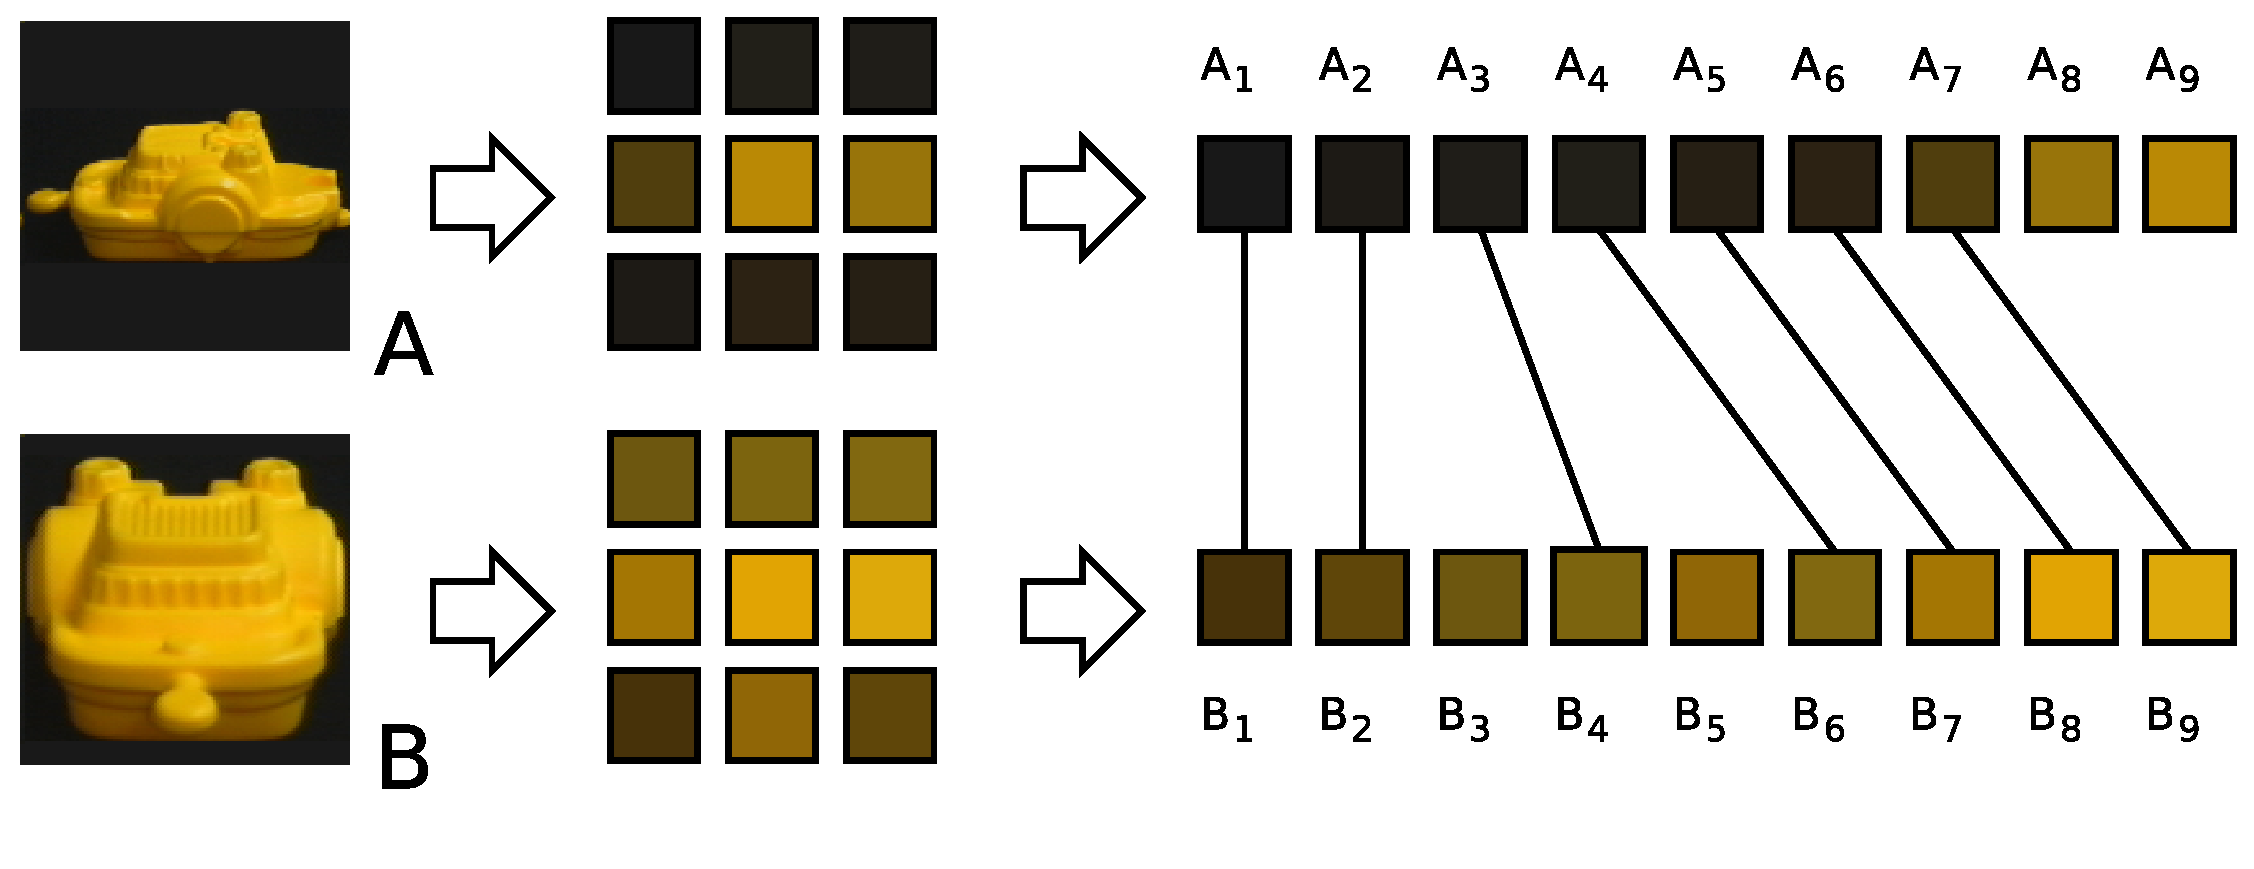
\includegraphics[width=10cm]{images/multires.eps}
\caption{\label{fig:multires}Constructie van een resolutie-onafhankelijke similariteitsmaat door gebruik van beeldonderdelen.}
\end{center}
\end{figure}

\begin{figure}[tbp]
\begin{center}
\subfigure[]{
\includegraphics[width=0.3\textwidth]{images/multires_sim-matrix_1.eps}
\label{fig:multires_sim-matrix_1}
}
\subfigure[]{
\includegraphics[width=0.3\textwidth]{images/multires_sim-matrix_2.eps}
\label{fig:multires_sim-matrix_2}
}
\subfigure[]{
\includegraphics[width=0.3\textwidth]{images/multires_sim-matrix_beide.eps}
\label{fig:multires_sim-matrix_beide}
}
\caption{\label{fig:multires_sim-matrices}Het pad in de similariteitsmatrix van de beelden uit 
figuur~\ref{fig:multires} voor (a) $M(A,B)$, (b) $M(B,A)$ en (c) beide.}
\end{center}
\end{figure}

%\begin{table}
%\begin{center}
%\begin{tabular}{|c|ccccccccc|}
%\hline
%$\scriptstyle M_3(A_i,B_j)$	& $B_1$ & $B_2$ & $B_3$ & $B_4$ & $B_5$ & $B_6$ & $B_7$ & $B_8$ & $B_9$  \\
%\hline
%$A_1$ 	& $\mathbf{\scriptstyle 0.5198}$ & $\scriptstyle 0.4496$ & & & & & & & \\
%$A_2$ 	& & $\mathbf{\scriptstyle 0.4691}$ & $\scriptstyle 0.3859$ & & & & & & \\
%$A_3$ 	& & & $\scriptstyle 0.4133$ & $\mathbf{\scriptstyle 0.4404}$ & $\scriptstyle 0.3298$ & & & & \\
%$A_4$ 	& & & & & $\scriptstyle 0.3277$ & $\mathbf{\scriptstyle 0.4330}$ & $\scriptstyle 0.3648$ & & \\
%$A_5$ 	& & & & & & & $\mathbf{\scriptstyle 0.3849}$ & $\scriptstyle 0.3134$ & \\
%$A_6$ 	& & & & & & & & $\mathbf{\scriptstyle 0.3438}$ & $\scriptstyle 0.3427$ \\
%$A_7$ 	& & & & & & & & & $\mathbf{\scriptstyle 0.5066}$ \\
%\hline
%\end{tabular}
%\caption{\label{tab:multires}De similariteiten die berekend worden in de constructie die ge\"illustreerd wordt door figuur~\ref{fig:multires}.}
%\end{center}
%\end{table}

We kunnen de similariteiten tussen de verschillende beeldonderdelen van twee beelden
samenbrengen in een \emph{similariteitsmatrix}. Een dergelijke matrix kan grafisch 
voorgesteld worden als een grijswaardebeeld, waarbij de waarde van een beeldpunt evenredig is met
de overeenkomstige similariteit. Figuur~\ref{fig:multires_sim-matrix_1} toont het pad in de 
similariteitsmatrix van de beelden $A$ en $B$ uit figuur~\ref{fig:multires}, dat wordt afgelopen
bij het bepalen van $M(A,B)$.
De similariteiten die effectief berekend worden, hebben in die figuur een volle rand. Diegene 
die toegevoegd worden aan $S$ hebben een dikkere rand. Die laatste similariteiten 
worden in figuur~\ref{fig:multires} weergegeven als volle verbindingen tussen de
geordende beeldonderdelen. 

Uit figuur~\ref{fig:multires_sim-matrices} blijkt inderdaad dat
het gemiddelde van $M(A,B)$ en $M(B,A)$ moet gebruikt worden om een symmetrische maat te bekomen.
De similariteiten die toegevoegd worden aan $S$ bij het berekenen van $M(B,A)$, worden in 
figuur~\ref{fig:multires} weergegeven met stippellijnen.


\section{Experimentele observaties}

%In figuur~\ref{fig:pixelgeb_gggrs_en_cputimes} 
Tot slot van dit hoofdstuk vergelijken we enkele pixelgebaseerde similariteitsmaten.
Hoewel de beelden in onze testcollectie allemaal dezelfde resolutie hebben, zullen de
resoluties van de beelden die we in de praktijk gaan vergelijken vrijwel altijd verschillend zijn.
We beperken ons daarom tot resolutie-onafhankelijke similariteitsmaten. Die maten construeren
we op basis van een pixelgebaseerde maat, zoals besproken in \ref{sectie:res-onafh}. 
Voor het toepassen van de vaagsimilariteitsmaten op
intermediaire beelden of op beeldonderdelen, beschouwen we de drie manieren uit \ref{sectie:kleurbeelden_similariteitsmaten}:
eerst omzetten naar grijswaardebeelden, 
toepassen op de afzonderlijke kleurcomponenten en 
de tralie-gebaseerde aanpak.

Figuur~\ref{fig:scaling_gggrs_en_cputimes} toont de GGGRs en de rekentijden voor de 
similariteitsmaten op basis van herschaling. De beste GGGR-waarde bekomen we in combinatie
met $M_7$. In figuur~\ref{fig:results_beste_scaling} worden de resultaten van die maat
weergegeven. Die resultaten zijn vrij goed, maar dat is slechts een vertekend beeld van de
werkelijkheid. De beelden in onze testcollectie hebben immers allemaal dezelfde resolutie,
waardoor er nooit herschaling nodig is. Als er wel herschaald moet worden, dan kunnen
eventuele vervormingen zorgen voor slechtere performantie. 

Een opvallende vastelling is dat de component-gebaseerde aanpak blijkbaar betere resultaten 
geeft dan de tralie-gebaseerde. Verkeerdelijk hoge similariteiten tussen sterk verschillende 
beelden zijn de oorzaak daarvan. Bij het vergelijken
van beelden die niet sterk verschillen kunnen dergelijke \emph{valse positieven} niet optreden.
Vandaar dat de tralie-gebaseerde aanpak wel goed kan presteren bij de constructie van
kwaliteitsmaten voor beelden \cite{debaets:similariteitsmaten_voor_kleurbeelden}.
Beschouw bijvoorbeeld twee beelden $A$ en $B$ die elk uit \'e\'en enkele pixel bestaan. De pixel 
van $A$ is rood en die van $B$ is groen, met andere woorden: $A((0,0))=(1,0,0)$ en 
$B((0,0))=(0,1,0)$. Er geldt dan: 
$$
|A_1|=1 \quad |A_2|=0 \quad |A_3|=0 \qquad |B_1|=0 \quad |B_2|=1 \quad |B_3|=0 \qquad |A|=|B|=\frac{\sqrt{1}}{\sqrt{3}}
$$
met $A(x)=(A_1(x),A_2(x),A_3(x))$ en $B(x)=(B_1(x),B_2(x),B_3(x))$ voor alle $x \in X$. Als we
$\frac{0}{0} = 0$ veronderstellen, dan geeft de component-gebaseerde aanpak dus
$$
\begin{array}{r@{\ =\ }l}
\displaystyle\frac{M_5(A_1,B_1)+M_5(A_2,B_2)+M_5(A_3,B_3)}{3} &
\displaystyle\frac{\frac{\min\{|A_1|,|B_1|\}}{\max\{|A_1|,|B_1|\}}+\frac{\min\{|A_2|,|B_2|\}}{\max\{|A_2|,|B_2|\}}+\frac{\min\{|A_3|,|B_3|\}}{\max\{|A_3|,|B_3|\}}}{3} \\[5pt]
 & \displaystyle\frac{\frac{0}{1}+\frac{0}{1}+0}{3} = 0
\end{array}
$$
terwijl we via de tralie-gebaseerde aanpak
$$
M_5(A,B) = \frac{\min\{|A|,|B|\}}{\max\{|A|,|B|\}} = \frac{\frac{\sqrt{1}}{\sqrt{3}}}{\frac{\sqrt{1}}{\sqrt{3}}} = 1
$$
bekomen. Voor de andere vaagsimilariteitsmaten die gebaseerd zijn op cardinaliteit, kunnen
analoge redeneringen gemaakt worden. De op afstand gebaseerde vaagsimilariteitsmaten ondervinden
minder hinder van dit probleem. Vandaar dat de tralie-gebaseerde aanpak in combinatie met
$M_{1a}$, $M_{1b}$, $M_{1c}$ of $M_{3}$ relatief gezien iets beter werkt. 

Als we de similariteiten berekenen op nieuwe intermediaire beelden van 8 pixels, die 
geconstrueerd worden met behulp van NeuQuant en Wu kwantisatie, dan bekomen we de
de meetresultaten die in figuur~\ref{fig:dom_colors_gggrs_en_cputimes} worden weergegeven.

%We gebruiken zowel NeuQuant als de Wu quantizer. De beeldonderdelen die we gebruiken bestaan 
%uit $8 \cdot 8 = 64$ pixels.

De component-gebaseerde aanpak in 
combinatie met $M_{I3c}$ geeft de GGGR-waarde $0.0240259$. Bij de tralie-gebaseerde aanpak
bekomen we de GGGR-waarde $0.0264069$ als we $M_{1a}$ gebruiken. De resultaten van deze
maten worden respectievelijk weergegeven in figuur~\ref{fig:results_beste_componenten_pixelgeb} en
figuur~\ref{fig:results_beste_tralie_pixelgeb}.
In die figuren zien we duidelijk dat de resultaten niet zo overtuigend zijn. Blijkbaar 
is de pixelgebaseerde benadering niet de meest geschikte voor image retrieval. 

Op het vlak van rekentijd zijn de similariteitsmaten op basis van de eerste en de laatste manier
aan elkaar gewaagd. Bij het toepassen van een similariteitsmaat voor grijswaardebeelden op de 
afzonderlijke kleurcomponenten, hebben we echter aanzienlijk meer rekentijd nodig. Dat is niet
verwonderlijk, aangezien er dan ook driemaal zoveel werk moet verricht worden.

\begin{figure}[tbp]
\begin{center}
\includegraphics[width=\textwidth]{plots/scaling_gggrs_en_cputimes_filled.eps}
\caption{\label{fig:scaling_gggrs_en_cputimes}De GGGR-waarde en de gebruikte rekentijd in ms voor elk van de resolutie-onafhankelijke pixelgebaseerde similariteitsmaten op basis van herschaalde beelden.}
\end{center}
\end{figure}

\begin{figure}[tbp]
\begin{center}
\begin{tabular}{m{11cm} | m{3cm} |}
\textbf{Eerste tien resultaten:} & \textbf{GGR:} \\
\vspace{4pt}
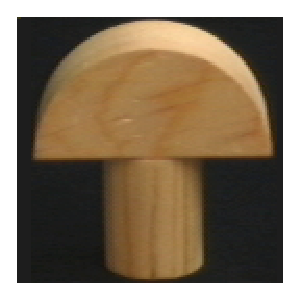
\includegraphics[width=1cm]{coil/beeld-0.eps}
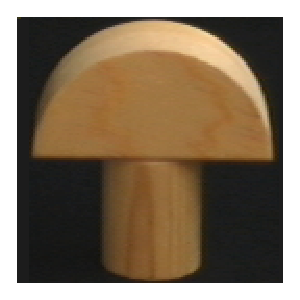
\includegraphics[width=1cm]{coil/beeld-1.eps}
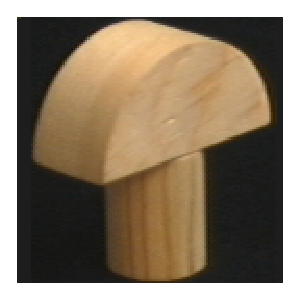
\includegraphics[width=1cm]{coil/beeld-3.eps}
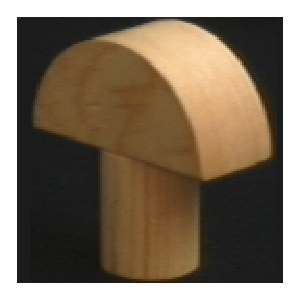
\includegraphics[width=1cm]{coil/beeld-4.eps}
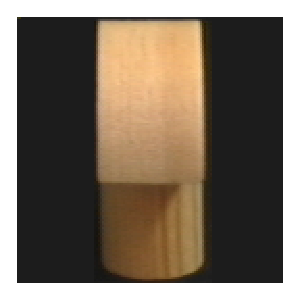
\includegraphics[width=1cm]{coil/beeld-2.eps}
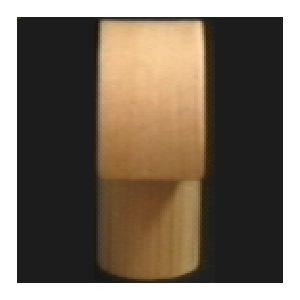
\includegraphics[width=1cm]{coil/beeld-5.eps}
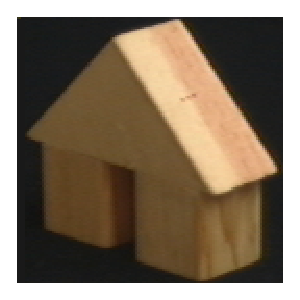
\includegraphics[width=1cm]{coil/beeld-46.eps}
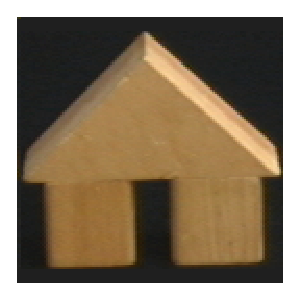
\includegraphics[width=1cm]{coil/beeld-42.eps}
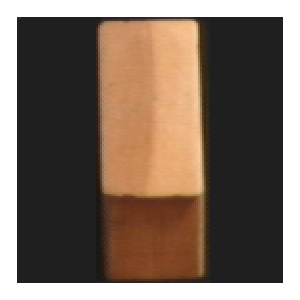
\includegraphics[width=1cm]{coil/beeld-44.eps}
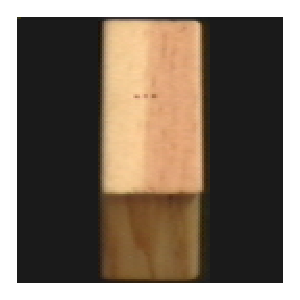
\includegraphics[width=1cm]{coil/beeld-47.eps}
& {\scriptsize 0.0}
\\
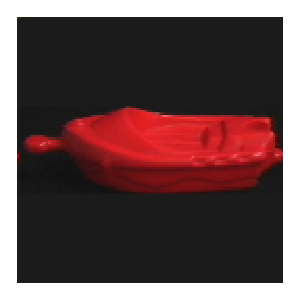
\includegraphics[width=1cm]{coil/beeld-18.eps}
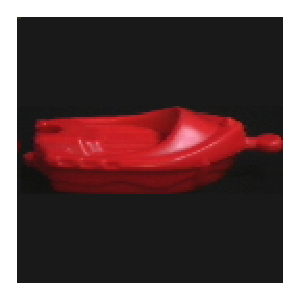
\includegraphics[width=1cm]{coil/beeld-19.eps}
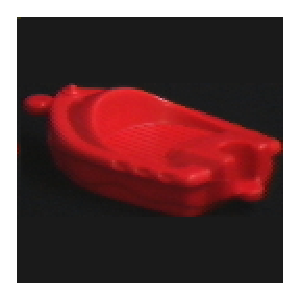
\includegraphics[width=1cm]{coil/beeld-22.eps}
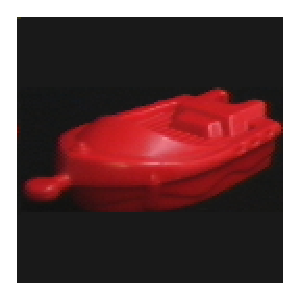
\includegraphics[width=1cm]{coil/beeld-21.eps}
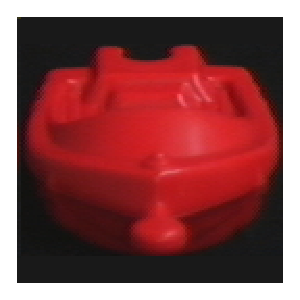
\includegraphics[width=1cm]{coil/beeld-20.eps}
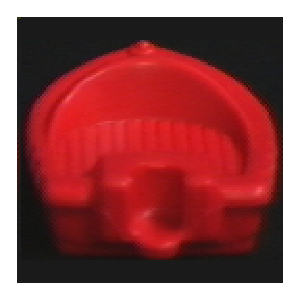
\includegraphics[width=1cm]{coil/beeld-23.eps}
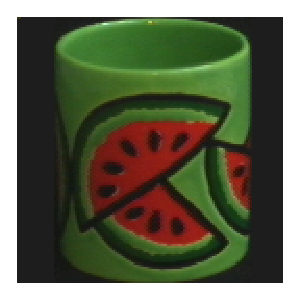
\includegraphics[width=1cm]{coil/beeld-32.eps}
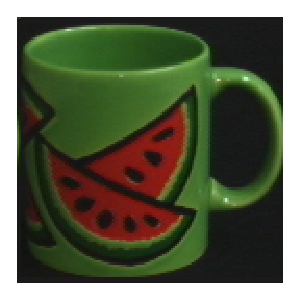
\includegraphics[width=1cm]{coil/beeld-30.eps}
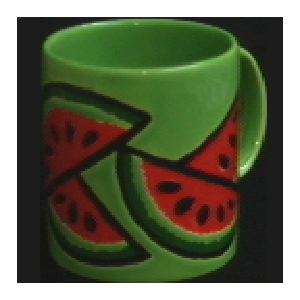
\includegraphics[width=1cm]{coil/beeld-33.eps}
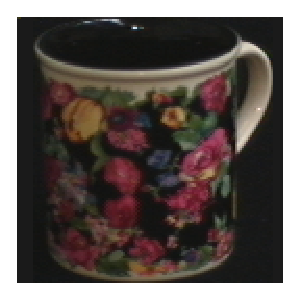
\includegraphics[width=1cm]{coil/beeld-63.eps}
& {\scriptsize 0.0}
\\
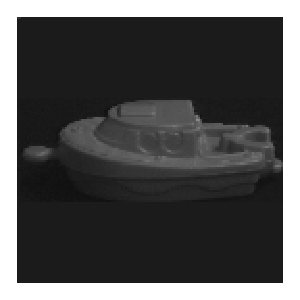
\includegraphics[width=1cm]{coil/beeld-24.eps}
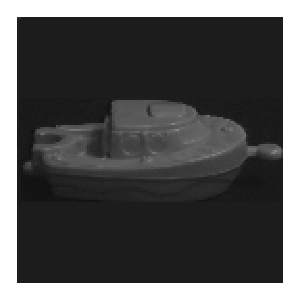
\includegraphics[width=1cm]{coil/beeld-25.eps}
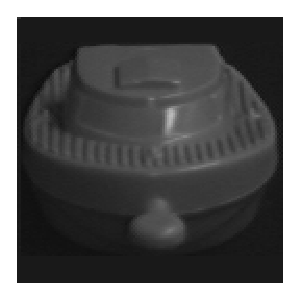
\includegraphics[width=1cm]{coil/beeld-28.eps}
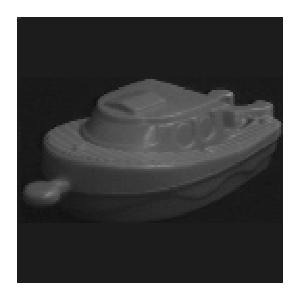
\includegraphics[width=1cm]{coil/beeld-27.eps}
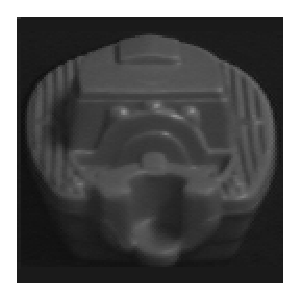
\includegraphics[width=1cm]{coil/beeld-26.eps}
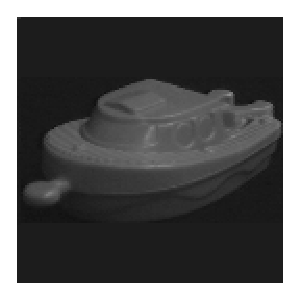
\includegraphics[width=1cm]{coil/beeld-29.eps}
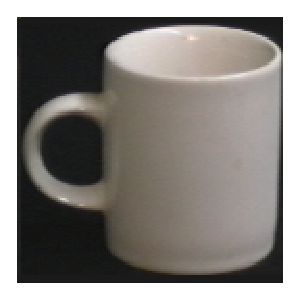
\includegraphics[width=1cm]{coil/beeld-37.eps}
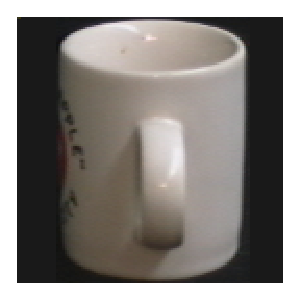
\includegraphics[width=1cm]{coil/beeld-41.eps}
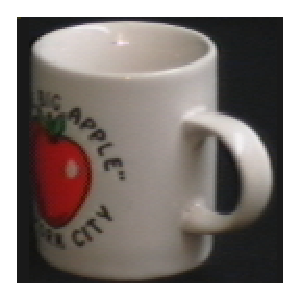
\includegraphics[width=1cm]{coil/beeld-40.eps}
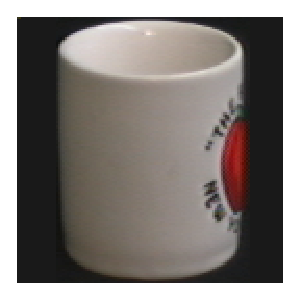
\includegraphics[width=1cm]{coil/beeld-38.eps}
& {\scriptsize 0.0}
\\
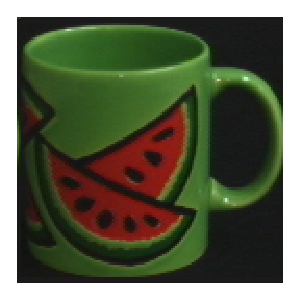
\includegraphics[width=1cm]{coil/beeld-30.eps}
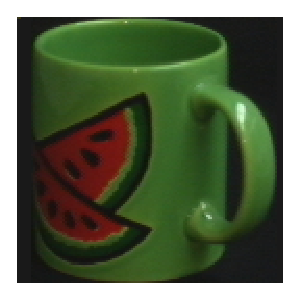
\includegraphics[width=1cm]{coil/beeld-34.eps}
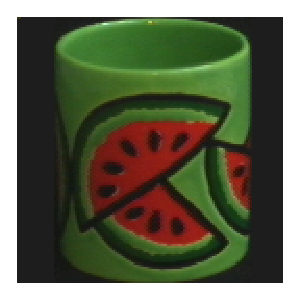
\includegraphics[width=1cm]{coil/beeld-32.eps}
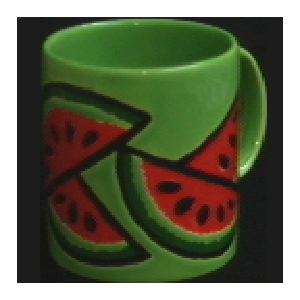
\includegraphics[width=1cm]{coil/beeld-33.eps}
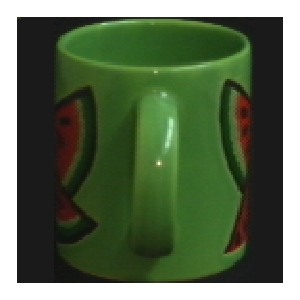
\includegraphics[width=1cm]{coil/beeld-35.eps}
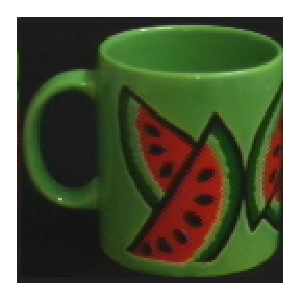
\includegraphics[width=1cm]{coil/beeld-31.eps}
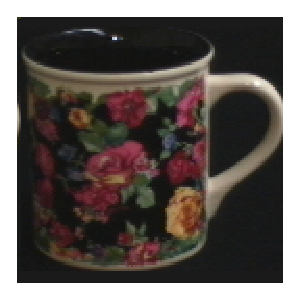
\includegraphics[width=1cm]{coil/beeld-60.eps}
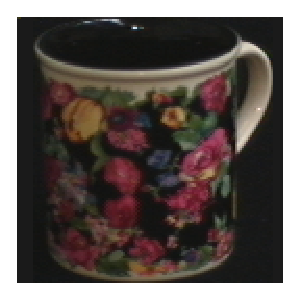
\includegraphics[width=1cm]{coil/beeld-63.eps}
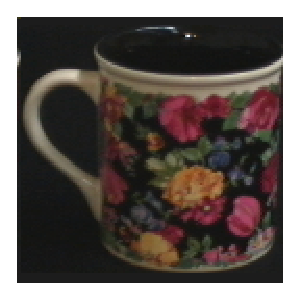
\includegraphics[width=1cm]{coil/beeld-61.eps}
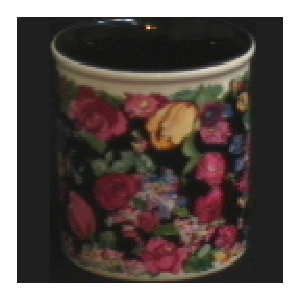
\includegraphics[width=1cm]{coil/beeld-62.eps}
& {\scriptsize 0.0}
\\
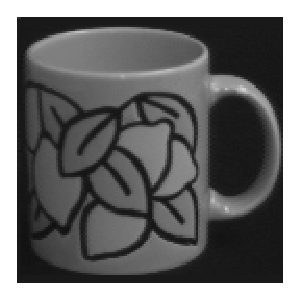
\includegraphics[width=1cm]{coil/beeld-48.eps}
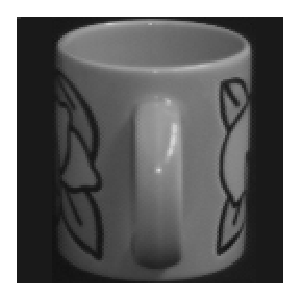
\includegraphics[width=1cm]{coil/beeld-50.eps}
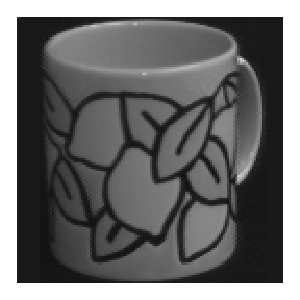
\includegraphics[width=1cm]{coil/beeld-51.eps}
\includegraphics[width=1cm]{coil/beeld-52.eps}
\includegraphics[width=1cm]{coil/beeld-53.eps}
\includegraphics[width=1cm]{coil/beeld-49.eps}
\includegraphics[width=1cm]{coil/beeld-29.eps}
\includegraphics[width=1cm]{coil/beeld-26.eps}
\includegraphics[width=1cm]{coil/beeld-27.eps}
\includegraphics[width=1cm]{coil/beeld-28.eps}
& {\scriptsize 0.0}
\\
\includegraphics[width=1cm]{coil/beeld-54.eps}
\includegraphics[width=1cm]{coil/beeld-55.eps}
\includegraphics[width=1cm]{coil/beeld-57.eps}
\includegraphics[width=1cm]{coil/beeld-58.eps}
\includegraphics[width=1cm]{coil/beeld-56.eps}
\includegraphics[width=1cm]{coil/beeld-59.eps}
\includegraphics[width=1cm]{coil/beeld-35.eps}
\includegraphics[width=1cm]{coil/beeld-34.eps}
\includegraphics[width=1cm]{coil/beeld-30.eps}
\includegraphics[width=1cm]{coil/beeld-33.eps}
& {\scriptsize 0.0}
\\
\includegraphics[width=1cm]{coil/beeld-6.eps}
\includegraphics[width=1cm]{coil/beeld-9.eps}
\includegraphics[width=1cm]{coil/beeld-8.eps}
\includegraphics[width=1cm]{coil/beeld-10.eps}
\includegraphics[width=1cm]{coil/beeld-11.eps}
\includegraphics[width=1cm]{coil/beeld-2.eps}
\includegraphics[width=1cm]{coil/beeld-36.eps}
\includegraphics[width=1cm]{coil/beeld-5.eps}
\includegraphics[width=1cm]{coil/beeld-7.eps}
\includegraphics[width=1cm]{coil/beeld-47.eps}
& {\scriptsize 0.007142857142857143}
\\
\includegraphics[width=1cm]{coil/beeld-60.eps}
\includegraphics[width=1cm]{coil/beeld-63.eps}
\includegraphics[width=1cm]{coil/beeld-61.eps}
\includegraphics[width=1cm]{coil/beeld-62.eps}
\includegraphics[width=1cm]{coil/beeld-30.eps}
\includegraphics[width=1cm]{coil/beeld-64.eps}
\includegraphics[width=1cm]{coil/beeld-32.eps}
\includegraphics[width=1cm]{coil/beeld-65.eps}
\includegraphics[width=1cm]{coil/beeld-33.eps}
\includegraphics[width=1cm]{coil/beeld-31.eps}
& {\scriptsize 0.007142857142857143}
\\
\includegraphics[width=1cm]{coil/beeld-36.eps}
\includegraphics[width=1cm]{coil/beeld-40.eps}
\includegraphics[width=1cm]{coil/beeld-39.eps}
\includegraphics[width=1cm]{coil/beeld-38.eps}
\includegraphics[width=1cm]{coil/beeld-10.eps}
\includegraphics[width=1cm]{coil/beeld-41.eps}
\includegraphics[width=1cm]{coil/beeld-3.eps}
\includegraphics[width=1cm]{coil/beeld-11.eps}
\includegraphics[width=1cm]{coil/beeld-6.eps}
\includegraphics[width=1cm]{coil/beeld-24.eps}
& {\scriptsize 0.016666666666666666}
\\
\includegraphics[width=1cm]{coil/beeld-42.eps}
\includegraphics[width=1cm]{coil/beeld-43.eps}
\includegraphics[width=1cm]{coil/beeld-46.eps}
\includegraphics[width=1cm]{coil/beeld-0.eps}
\includegraphics[width=1cm]{coil/beeld-45.eps}
\includegraphics[width=1cm]{coil/beeld-3.eps}
\includegraphics[width=1cm]{coil/beeld-1.eps}
\includegraphics[width=1cm]{coil/beeld-4.eps}
\includegraphics[width=1cm]{coil/beeld-2.eps}
\includegraphics[width=1cm]{coil/beeld-10.eps}
& {\scriptsize 0.0380952380952381}
\\
\includegraphics[width=1cm]{coil/beeld-12.eps}
\includegraphics[width=1cm]{coil/beeld-13.eps}
\includegraphics[width=1cm]{coil/beeld-16.eps}
\includegraphics[width=1cm]{coil/beeld-15.eps}
\includegraphics[width=1cm]{coil/beeld-21.eps}
\includegraphics[width=1cm]{coil/beeld-22.eps}
\includegraphics[width=1cm]{coil/beeld-18.eps}
\includegraphics[width=1cm]{coil/beeld-19.eps}
\includegraphics[width=1cm]{coil/beeld-30.eps}
\includegraphics[width=1cm]{coil/beeld-33.eps}
& {\scriptsize 0.15}
\\
\end{tabular}
\caption{\label{fig:results_beste_scaling}De GGR-waarde en de eerste tien resultaten voor elk voorbeeld bij de resolutie-onafhankelijke similariteitsmaat die we bekomen door herschaalde beelden componentsgewijs te vergelijken met behulp van $M_7$.}
\end{center}
\end{figure}

\begin{figure}[tbp]
\begin{center}
\subfigure[]{
\begin{minipage}{\textwidth}
\includegraphics[width=\textwidth]{plots/dom_colors_neuquant_gggrs_en_cputimes_filled.eps}
\vspace{2pt}
\end{minipage}
\label{fig:dom_colors_neuquant_gggrs_en_cputimes}
}
\subfigure[]{
\begin{minipage}{\textwidth}
\includegraphics[width=\textwidth]{plots/dom_colors_wu_gggrs_en_cputimes_filled.eps}
\vspace{2pt}
\end{minipage}
\label{fig:dom_colors_wu_gggrs_en_cputimes}
}
\caption{\label{fig:dom_colors_gggrs_en_cputimes}De GGGR-waarde en de gebruikte rekentijd in ms voor elk van de resolutie-onafhankelijke pixelgebaseerde similariteitsmaten op basis van nieuwe geconstrueerde intermediaire beelden met (a) NeuQuant en (b) Wu kwantisatie.}
\end{center}
\end{figure}

\begin{figure}[!p]
\begin{center}
\begin{tabular}{m{11cm} | m{3cm} |}
\textbf{Eerste tien resultaten:} & \textbf{GGR:} \\
\vspace{4pt}
\includegraphics[width=1cm]{coil/beeld-12.eps}
\includegraphics[width=1cm]{coil/beeld-17.eps}
\includegraphics[width=1cm]{coil/beeld-13.eps}
\includegraphics[width=1cm]{coil/beeld-15.eps}
\includegraphics[width=1cm]{coil/beeld-14.eps}
\includegraphics[width=1cm]{coil/beeld-16.eps}
\includegraphics[width=1cm]{coil/beeld-42.eps}
\includegraphics[width=1cm]{coil/beeld-5.eps}
\includegraphics[width=1cm]{coil/beeld-4.eps}
\includegraphics[width=1cm]{coil/beeld-1.eps}
& {\scriptsize 0.0}
\\
\includegraphics[width=1cm]{coil/beeld-18.eps}
\includegraphics[width=1cm]{coil/beeld-20.eps}
\includegraphics[width=1cm]{coil/beeld-23.eps}
\includegraphics[width=1cm]{coil/beeld-22.eps}
\includegraphics[width=1cm]{coil/beeld-21.eps}
\includegraphics[width=1cm]{coil/beeld-19.eps}
\includegraphics[width=1cm]{coil/beeld-45.eps}
\includegraphics[width=1cm]{coil/beeld-31.eps}
\includegraphics[width=1cm]{coil/beeld-30.eps}
\includegraphics[width=1cm]{coil/beeld-33.eps}
& {\scriptsize 0.0}
\\
\includegraphics[width=1cm]{coil/beeld-30.eps}
\includegraphics[width=1cm]{coil/beeld-31.eps}
\includegraphics[width=1cm]{coil/beeld-33.eps}
\includegraphics[width=1cm]{coil/beeld-32.eps}
\includegraphics[width=1cm]{coil/beeld-35.eps}
\includegraphics[width=1cm]{coil/beeld-34.eps}
\includegraphics[width=1cm]{coil/beeld-61.eps}
\includegraphics[width=1cm]{coil/beeld-60.eps}
\includegraphics[width=1cm]{coil/beeld-63.eps}
\includegraphics[width=1cm]{coil/beeld-62.eps}
& {\scriptsize 0.0}
\\
\includegraphics[width=1cm]{coil/beeld-54.eps}
\includegraphics[width=1cm]{coil/beeld-58.eps}
\includegraphics[width=1cm]{coil/beeld-59.eps}
\includegraphics[width=1cm]{coil/beeld-56.eps}
\includegraphics[width=1cm]{coil/beeld-55.eps}
\includegraphics[width=1cm]{coil/beeld-57.eps}
\includegraphics[width=1cm]{coil/beeld-35.eps}
\includegraphics[width=1cm]{coil/beeld-34.eps}
\includegraphics[width=1cm]{coil/beeld-32.eps}
\includegraphics[width=1cm]{coil/beeld-33.eps}
& {\scriptsize 0.0}
\\
\includegraphics[width=1cm]{coil/beeld-24.eps}
\includegraphics[width=1cm]{coil/beeld-28.eps}
\includegraphics[width=1cm]{coil/beeld-29.eps}
\includegraphics[width=1cm]{coil/beeld-25.eps}
\includegraphics[width=1cm]{coil/beeld-27.eps}
\includegraphics[width=1cm]{coil/beeld-37.eps}
\includegraphics[width=1cm]{coil/beeld-41.eps}
\includegraphics[width=1cm]{coil/beeld-26.eps}
\includegraphics[width=1cm]{coil/beeld-48.eps}
\includegraphics[width=1cm]{coil/beeld-51.eps}
& {\scriptsize 0.004761904761904762}
\\
\includegraphics[width=1cm]{coil/beeld-48.eps}
\includegraphics[width=1cm]{coil/beeld-51.eps}
\includegraphics[width=1cm]{coil/beeld-50.eps}
\includegraphics[width=1cm]{coil/beeld-52.eps}
\includegraphics[width=1cm]{coil/beeld-26.eps}
\includegraphics[width=1cm]{coil/beeld-49.eps}
\includegraphics[width=1cm]{coil/beeld-27.eps}
\includegraphics[width=1cm]{coil/beeld-53.eps}
\includegraphics[width=1cm]{coil/beeld-37.eps}
\includegraphics[width=1cm]{coil/beeld-25.eps}
& {\scriptsize 0.007142857142857143}
\\
\includegraphics[width=1cm]{coil/beeld-60.eps}
\includegraphics[width=1cm]{coil/beeld-63.eps}
\includegraphics[width=1cm]{coil/beeld-62.eps}
\includegraphics[width=1cm]{coil/beeld-61.eps}
\includegraphics[width=1cm]{coil/beeld-7.eps}
\includegraphics[width=1cm]{coil/beeld-64.eps}
\includegraphics[width=1cm]{coil/beeld-8.eps}
\includegraphics[width=1cm]{coil/beeld-9.eps}
\includegraphics[width=1cm]{coil/beeld-65.eps}
\includegraphics[width=1cm]{coil/beeld-0.eps}
& {\scriptsize 0.009523809523809525}
\\
\includegraphics[width=1cm]{coil/beeld-6.eps}
\includegraphics[width=1cm]{coil/beeld-10.eps}
\includegraphics[width=1cm]{coil/beeld-40.eps}
\includegraphics[width=1cm]{coil/beeld-65.eps}
\includegraphics[width=1cm]{coil/beeld-11.eps}
\includegraphics[width=1cm]{coil/beeld-38.eps}
\includegraphics[width=1cm]{coil/beeld-9.eps}
\includegraphics[width=1cm]{coil/beeld-39.eps}
\includegraphics[width=1cm]{coil/beeld-8.eps}
\includegraphics[width=1cm]{coil/beeld-64.eps}
& {\scriptsize 0.0380952380952381}
\\
\includegraphics[width=1cm]{coil/beeld-0.eps}
\includegraphics[width=1cm]{coil/beeld-2.eps}
\includegraphics[width=1cm]{coil/beeld-46.eps}
\includegraphics[width=1cm]{coil/beeld-44.eps}
\includegraphics[width=1cm]{coil/beeld-45.eps}
\includegraphics[width=1cm]{coil/beeld-1.eps}
\includegraphics[width=1cm]{coil/beeld-43.eps}
\includegraphics[width=1cm]{coil/beeld-47.eps}
\includegraphics[width=1cm]{coil/beeld-3.eps}
\includegraphics[width=1cm]{coil/beeld-4.eps}
& {\scriptsize 0.04523809523809524}
\\
\includegraphics[width=1cm]{coil/beeld-36.eps}
\includegraphics[width=1cm]{coil/beeld-11.eps}
\includegraphics[width=1cm]{coil/beeld-40.eps}
\includegraphics[width=1cm]{coil/beeld-39.eps}
\includegraphics[width=1cm]{coil/beeld-38.eps}
\includegraphics[width=1cm]{coil/beeld-10.eps}
\includegraphics[width=1cm]{coil/beeld-6.eps}
\includegraphics[width=1cm]{coil/beeld-46.eps}
\includegraphics[width=1cm]{coil/beeld-41.eps}
\includegraphics[width=1cm]{coil/beeld-47.eps}
& {\scriptsize 0.047619047619047616}
\\
\includegraphics[width=1cm]{coil/beeld-42.eps}
\includegraphics[width=1cm]{coil/beeld-5.eps}
\includegraphics[width=1cm]{coil/beeld-4.eps}
\includegraphics[width=1cm]{coil/beeld-3.eps}
\includegraphics[width=1cm]{coil/beeld-43.eps}
\includegraphics[width=1cm]{coil/beeld-47.eps}
\includegraphics[width=1cm]{coil/beeld-1.eps}
\includegraphics[width=1cm]{coil/beeld-46.eps}
\includegraphics[width=1cm]{coil/beeld-44.eps}
\includegraphics[width=1cm]{coil/beeld-2.eps}
& {\scriptsize 0.047619047619047616}
\\
\end{tabular}
\caption{\label{fig:results_beste_dom_colors}De GGR-waarde en de eerste tien resultaten voor elk voorbeeld bij de resolutie-onafhankelijke similariteitsmaat die we bekomen door nieuwe geconstrueerde intermediaire beelden componentsgewijs te vergelijken met behulp van $M_5$.}
\end{center}
\end{figure}

\begin{figure}[!t]
\begin{center}
\includegraphics[width=\textwidth]{plots/multires_gggrs_en_cputimes_filled.eps}
\caption{\label{fig:multires_gggrs_en_cputimes}De GGGR-waarde en de gebruikte rekentijd in ms voor elk van de resolutie-onafhankelijke pixelgebaseerde similariteitsmaten op basis van beeldonderdelen.}
\end{center}
\end{figure}

\begin{figure}[tbp]
\begin{center}
\begin{tabular}{m{11cm} | m{3cm} |}
\textbf{Eerste tien resultaten:} & \textbf{GGR:} \\
\vspace{4pt}
\includegraphics[width=1cm]{coil/beeld-18.eps}
\includegraphics[width=1cm]{coil/beeld-22.eps}
\includegraphics[width=1cm]{coil/beeld-21.eps}
\includegraphics[width=1cm]{coil/beeld-19.eps}
\includegraphics[width=1cm]{coil/beeld-20.eps}
\includegraphics[width=1cm]{coil/beeld-23.eps}
\includegraphics[width=1cm]{coil/beeld-61.eps}
\includegraphics[width=1cm]{coil/beeld-63.eps}
\includegraphics[width=1cm]{coil/beeld-62.eps}
\includegraphics[width=1cm]{coil/beeld-60.eps}
& {\scriptsize 0.0}
\\
\includegraphics[width=1cm]{coil/beeld-24.eps}
\includegraphics[width=1cm]{coil/beeld-25.eps}
\includegraphics[width=1cm]{coil/beeld-28.eps}
\includegraphics[width=1cm]{coil/beeld-27.eps}
\includegraphics[width=1cm]{coil/beeld-26.eps}
\includegraphics[width=1cm]{coil/beeld-29.eps}
\includegraphics[width=1cm]{coil/beeld-10.eps}
\includegraphics[width=1cm]{coil/beeld-38.eps}
\includegraphics[width=1cm]{coil/beeld-11.eps}
\includegraphics[width=1cm]{coil/beeld-9.eps}
& {\scriptsize 0.0}
\\
\includegraphics[width=1cm]{coil/beeld-30.eps}
\includegraphics[width=1cm]{coil/beeld-34.eps}
\includegraphics[width=1cm]{coil/beeld-35.eps}
\includegraphics[width=1cm]{coil/beeld-31.eps}
\includegraphics[width=1cm]{coil/beeld-33.eps}
\includegraphics[width=1cm]{coil/beeld-32.eps}
\includegraphics[width=1cm]{coil/beeld-55.eps}
\includegraphics[width=1cm]{coil/beeld-61.eps}
\includegraphics[width=1cm]{coil/beeld-54.eps}
\includegraphics[width=1cm]{coil/beeld-60.eps}
& {\scriptsize 0.0}
\\
\includegraphics[width=1cm]{coil/beeld-36.eps}
\includegraphics[width=1cm]{coil/beeld-38.eps}
\includegraphics[width=1cm]{coil/beeld-41.eps}
\includegraphics[width=1cm]{coil/beeld-37.eps}
\includegraphics[width=1cm]{coil/beeld-27.eps}
\includegraphics[width=1cm]{coil/beeld-39.eps}
\includegraphics[width=1cm]{coil/beeld-4.eps}
\includegraphics[width=1cm]{coil/beeld-40.eps}
\includegraphics[width=1cm]{coil/beeld-24.eps}
\includegraphics[width=1cm]{coil/beeld-11.eps}
& {\scriptsize 0.007142857142857143}
\\
\includegraphics[width=1cm]{coil/beeld-48.eps}
\includegraphics[width=1cm]{coil/beeld-27.eps}
\includegraphics[width=1cm]{coil/beeld-53.eps}
\includegraphics[width=1cm]{coil/beeld-50.eps}
\includegraphics[width=1cm]{coil/beeld-52.eps}
\includegraphics[width=1cm]{coil/beeld-51.eps}
\includegraphics[width=1cm]{coil/beeld-49.eps}
\includegraphics[width=1cm]{coil/beeld-26.eps}
\includegraphics[width=1cm]{coil/beeld-28.eps}
\includegraphics[width=1cm]{coil/beeld-29.eps}
& {\scriptsize 0.011904761904761904}
\\
\includegraphics[width=1cm]{coil/beeld-12.eps}
\includegraphics[width=1cm]{coil/beeld-13.eps}
\includegraphics[width=1cm]{coil/beeld-15.eps}
\includegraphics[width=1cm]{coil/beeld-16.eps}
\includegraphics[width=1cm]{coil/beeld-30.eps}
\includegraphics[width=1cm]{coil/beeld-20.eps}
\includegraphics[width=1cm]{coil/beeld-34.eps}
\includegraphics[width=1cm]{coil/beeld-31.eps}
\includegraphics[width=1cm]{coil/beeld-17.eps}
\includegraphics[width=1cm]{coil/beeld-14.eps}
& {\scriptsize 0.01904761904761905}
\\
\includegraphics[width=1cm]{coil/beeld-54.eps}
\includegraphics[width=1cm]{coil/beeld-55.eps}
\includegraphics[width=1cm]{coil/beeld-57.eps}
\includegraphics[width=1cm]{coil/beeld-58.eps}
\includegraphics[width=1cm]{coil/beeld-34.eps}
\includegraphics[width=1cm]{coil/beeld-31.eps}
\includegraphics[width=1cm]{coil/beeld-30.eps}
\includegraphics[width=1cm]{coil/beeld-35.eps}
\includegraphics[width=1cm]{coil/beeld-59.eps}
\includegraphics[width=1cm]{coil/beeld-56.eps}
& {\scriptsize 0.01904761904761905}
\\
\includegraphics[width=1cm]{coil/beeld-60.eps}
\includegraphics[width=1cm]{coil/beeld-61.eps}
\includegraphics[width=1cm]{coil/beeld-63.eps}
\includegraphics[width=1cm]{coil/beeld-62.eps}
\includegraphics[width=1cm]{coil/beeld-30.eps}
\includegraphics[width=1cm]{coil/beeld-34.eps}
\includegraphics[width=1cm]{coil/beeld-31.eps}
\includegraphics[width=1cm]{coil/beeld-64.eps}
\includegraphics[width=1cm]{coil/beeld-35.eps}
\includegraphics[width=1cm]{coil/beeld-33.eps}
& {\scriptsize 0.02142857142857143}
\\
\includegraphics[width=1cm]{coil/beeld-0.eps}
\includegraphics[width=1cm]{coil/beeld-1.eps}
\includegraphics[width=1cm]{coil/beeld-42.eps}
\includegraphics[width=1cm]{coil/beeld-5.eps}
\includegraphics[width=1cm]{coil/beeld-43.eps}
\includegraphics[width=1cm]{coil/beeld-2.eps}
\includegraphics[width=1cm]{coil/beeld-44.eps}
\includegraphics[width=1cm]{coil/beeld-4.eps}
\includegraphics[width=1cm]{coil/beeld-64.eps}
\includegraphics[width=1cm]{coil/beeld-3.eps}
& {\scriptsize 0.023809523809523808}
\\
\includegraphics[width=1cm]{coil/beeld-6.eps}
\includegraphics[width=1cm]{coil/beeld-64.eps}
\includegraphics[width=1cm]{coil/beeld-7.eps}
\includegraphics[width=1cm]{coil/beeld-8.eps}
\includegraphics[width=1cm]{coil/beeld-65.eps}
\includegraphics[width=1cm]{coil/beeld-9.eps}
\includegraphics[width=1cm]{coil/beeld-25.eps}
\includegraphics[width=1cm]{coil/beeld-24.eps}
\includegraphics[width=1cm]{coil/beeld-60.eps}
\includegraphics[width=1cm]{coil/beeld-61.eps}
& {\scriptsize 0.06190476190476191}
\\
\includegraphics[width=1cm]{coil/beeld-42.eps}
\includegraphics[width=1cm]{coil/beeld-0.eps}
\includegraphics[width=1cm]{coil/beeld-1.eps}
\includegraphics[width=1cm]{coil/beeld-5.eps}
\includegraphics[width=1cm]{coil/beeld-43.eps}
\includegraphics[width=1cm]{coil/beeld-3.eps}
\includegraphics[width=1cm]{coil/beeld-2.eps}
\includegraphics[width=1cm]{coil/beeld-44.eps}
\includegraphics[width=1cm]{coil/beeld-4.eps}
\includegraphics[width=1cm]{coil/beeld-64.eps}
& {\scriptsize 0.1}
\\
\end{tabular}
\caption{\label{fig:results_beste_componenten_pixelgeb}De GGR-waarde en de eerste tien resultaten voor elk voorbeeld bij de resolutie-onafhankelijke similariteitsmaat die we bekomen door beeldonderdelen componentsgewijs te vergelijken met behulp van $M_{I3c}$.}
\end{center}
\end{figure}
